% !TeX root = main.tex

\section{Q2: Jacobian of 3R Spatial Manipulator}

\subsection*{Forward Kinematics}

The 3R spatial manipulator (joints in ortho-parallel configuration) can be through of as a 2R manipulator (formed by the last two joints) embed in a plane and that plane itself being able to rotate (because of the first joint).

\begin{figure}[ht]
    \centering
    \begin{subfigure}[b]{0.4 \textwidth}
        \centering
        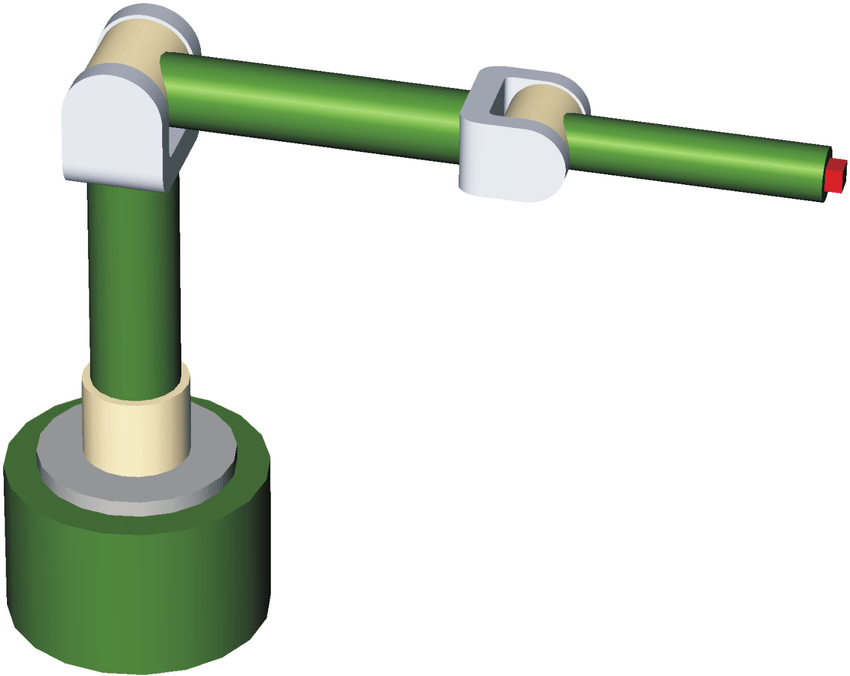
\includegraphics[width=\textwidth]{3r-op-manip.png}
        \caption{Manipulator}
        \label{fig:sfig-3r-op-manip}
    \end{subfigure}
    \begin{subfigure}[b]{0.4 \textwidth}
        \centering
        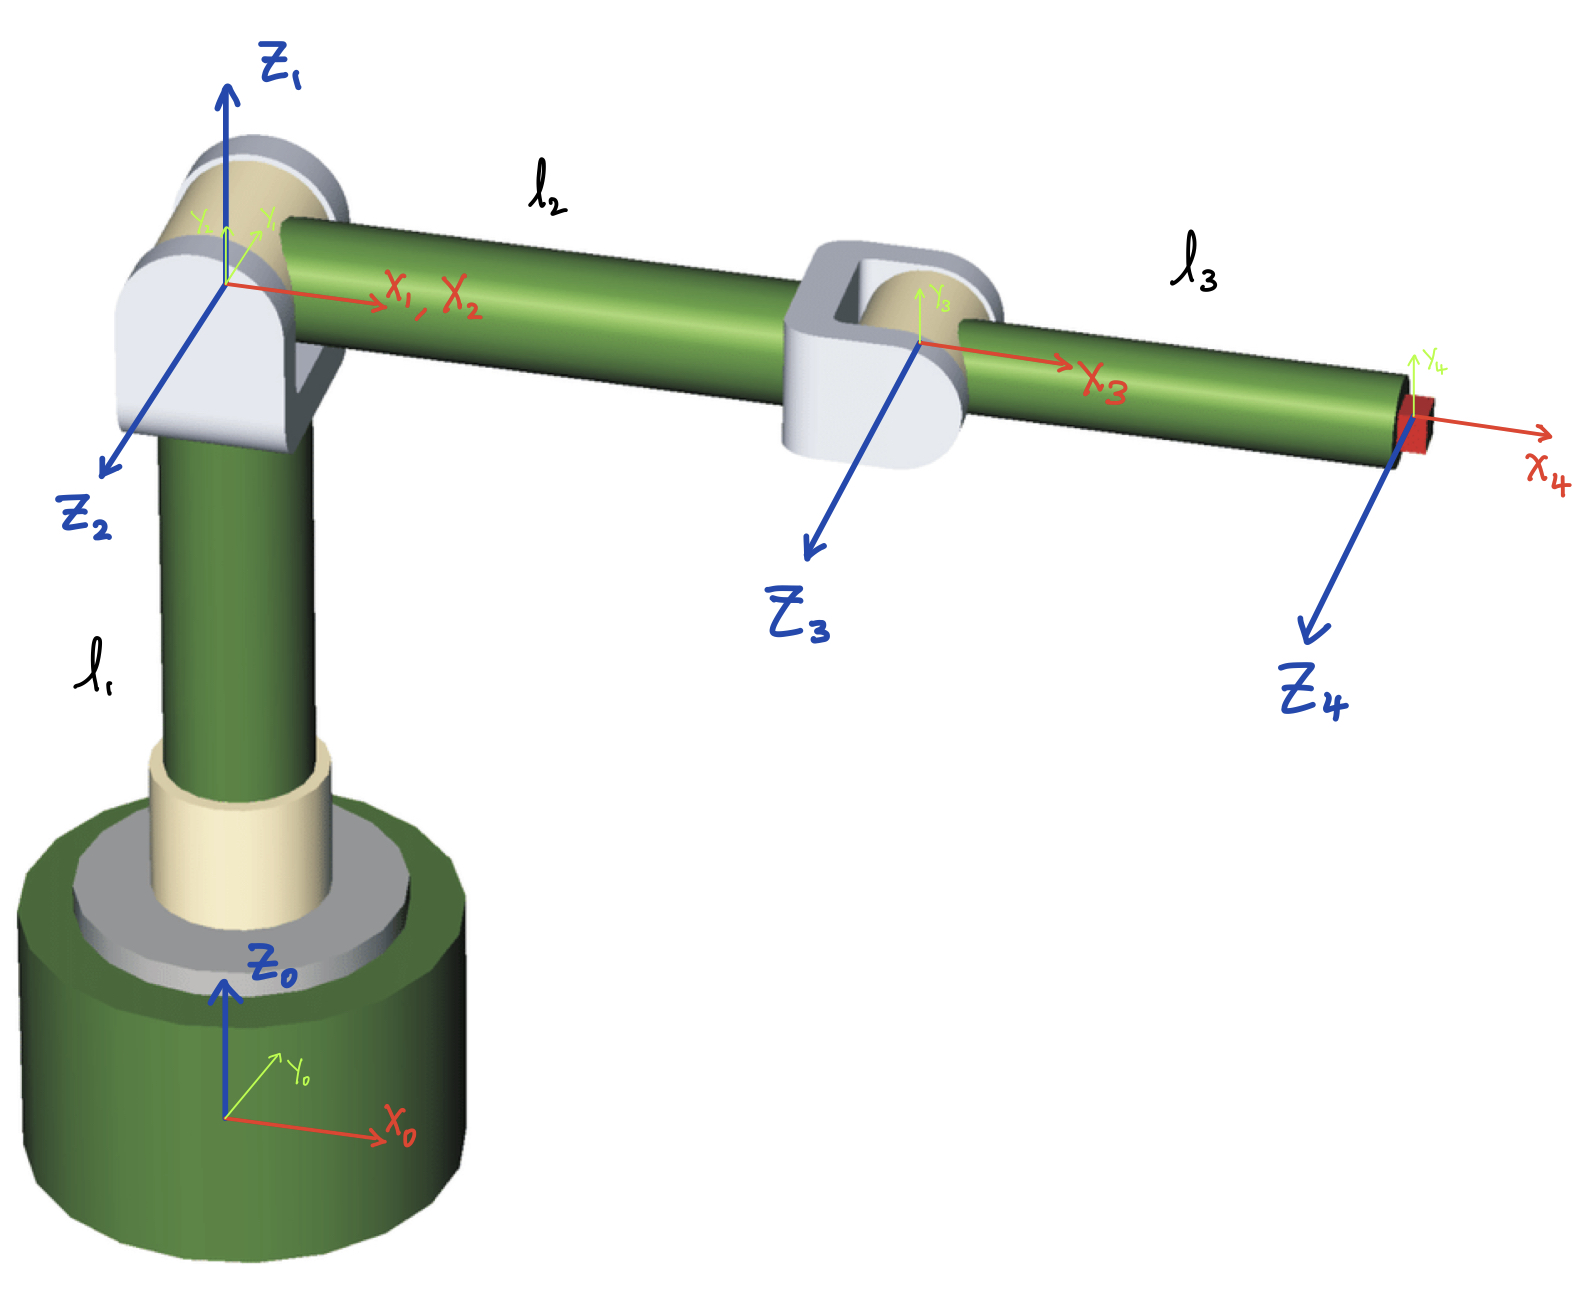
\includegraphics[width=\textwidth]{3r-fk-dh.png}
        \caption{Frame assignment}
        \label{fig:sfig-3r-op-frames}
    \end{subfigure}
    \caption{3R ortho-parallel manipulator}
    \label{fig:3r-op-manip-frames}
    \small
        On the left (\ref{sub@fig:sfig-3r-op-manip}) is the 3R ortho-parallel manipulator and on the right (\ref{sub@fig:sfig-3r-op-frames}) is the frame assignment using the modern DH convention.
\end{figure}

The DH parameters are shown in table \ref{tab:3r-op-dh-params}.

\begin{table}[h]
    \centering
    \begin{tabular}{ || c || c | c | c | c || }
        \hline
        $i$ & $\alpha_{i-1}$ & $a_{i-1}$ & $\theta_{i}$ & $d_{i}$ \\
        \hline \hline
        1 & 0 & 0 & $\theta_1$ & $l_1$ \\
        \hline
        2 & $\pi / 2$ & 0 & $\theta_2$ & 0 \\
        \hline
        3 & 0 & $l_2$ & $\theta_3$ & 0 \\
        \hline
        4 & 0 & $l_3$ & 0 & 0 \\
        \hline
    \end{tabular}
    \caption{DH Parameters of 3R ortho-parallel manipulator}
    \label{tab:3r-op-dh-params}
\end{table}

The forward kinematics are derived through the equations below

\begin{align}
    ^{0}_{1}\mathbf{T} = \begin{bmatrix}
        c_1 & -s_1 & 0 & 0 \\
        s_1 & c_1 & 0 & 0 \\
        0 & 0 & 1 & l_1 \\
        0 & 0 & 0 & 1
        \end{bmatrix}
    &&
    ^{1}_{2}\mathbf{T} = \begin{bmatrix}
        c_2 & -s_2 & 0 & 0 \\
        0 & 0 & -1 & 0 \\
        s_2 & c_2 & 0 & 0 \\
        0 & 0 & 0 & 1
        \end{bmatrix}
    &&
    ^{2}_{3}\mathbf{T} = \begin{bmatrix}
        c_3 & -s_3 & 0 & l_2 \\
        s_3 & c_3 & 0 & 0 \\
        0 & 0 & 1 & 0 \\
        0 & 0 & 0 & 1
        \end{bmatrix}
    &&
    ^{3}_{4}\mathbf{T} = \begin{bmatrix}
        1 & 0 & 0 & l_3 \\
        0 & 1 & 0 & 0 \\
        0 & 0 & 1 & 0 \\
        0 & 0 & 0 & 1
        \end{bmatrix}
    \nonumber
\end{align}

\begin{align}
    ^{0}_{2}\mathbf{T} = \begin{bmatrix}
        c_1 c_2 & -s_2 c_1 & s_1 & 0 \\
        s_1 c_2 & -s_1 s_2 & -c_1 & 0 \\
        s_2 & c_2 & 0 & l_1 \\
        0 & 0 & 0 & 1
        \end{bmatrix} &&
    ^{0}_{3}\mathbf{T} = \begin{bmatrix}
        c_1 c_{23} & -s_{23} c_1 & s_1 & l_2 c_1 c_2 \\
        s_1 c_{23} & -s_1 s_{23} & -c_1 & l_2 s_1 c_2 \\
        s_{23} & c_{23} & 0 & l_1 +l_2 s_2 \\
        0 & 0 & 0 & 1
        \end{bmatrix}
    \label{eq:3r-op-tfs-0}
\end{align}

Which gives

\begin{equation}
    ^{0}_{4}\mathbf{T} = \begin{bmatrix}
        c_1 c_{23} & -s_{23} c_1 & s_1 & (l_2 c_2 + l_3 c_{23})c_1 \\
        s_1 c_{23} & -s_1 s_{23} & -c_1 & (l_2 c_2 + l_3 c_{23})s_1 \\
        s_{23} & c_{23} & 0 & l_1 + l_2s_2 + l_3s_{23} \\
        0 & 0 & 0 & 1
    \end{bmatrix}
    \label{eq:3r-op-end-tf}
\end{equation}

For the angular velocity, we use the Z axis and the rotation matrices of the transforms obtained above.

\subsection{Velocity Jacobian}

The position of the end effector in the scene is (from equation \ref{eq:3r-op-end-tf})

\begin{align}
    \mathbf{p} = \begin{bmatrix}
        (l_2 c_2 + l_3 c_{23})c_1 \\
        (l_2 c_2 + l_3 c_{23})s_1 \\
        l_1 + l_2s_2 + l_3s_{23}
        \end{bmatrix} && \mathbf{v} = \dot{\mathbf{p}} = \mathbf{J_v} \begin{bmatrix}
            \dot{\theta_1} \\ \dot{\theta_2} \\ \dot{\theta_3}
            \end{bmatrix}
    \nonumber \\
    \mathbf{J_v} = \begin{bmatrix}
        -(l_2c_2 + l_3c_{23})s_1 & -(l_2s_2 + l_3s_{23})c_1 & l_3s_{23}c_1 \\
        (l_2c_2 + l_3c_{23})c_1 & -(l_2s_2 + l_3s_{23})s_1 & l_3s_1s_{23} \\
        0 & l_2c_2+l_3c_{23} & l_3 c_{23}
        \end{bmatrix}
    \label{eq:3r-op-jv}
\end{align}

The equation \ref{eq:3r-op-jv} gives the jacobian for the linear velocity part.

\subsection{Angular Velocity Jacobian}

The angular velocity of the end effector (along XYZ axis) is given by the vector

\begin{align}
    \mathbf{\Omega} &= \begin{bmatrix}
        \omega_x \\ \omega_y \\ \omega_z
        \end{bmatrix} = \begin{bmatrix}
        _0\textup{Z}_1 & _0\textup{Z}_2 & _0\textup{Z}_3
        \end{bmatrix} \begin{bmatrix}
        \dot{\theta_1} \\ \dot{\theta_2} \\ \dot{\theta_3}
        \end{bmatrix} = \begin{bmatrix}
        ^0_1\mathbf{R} \, \textup{Z} & ^0_2\mathbf{R} \, \textup{Z} & ^0_3\mathbf{R} \, \textup{Z}
        \end{bmatrix} \begin{bmatrix}
        \dot{\theta_1} \\ \dot{\theta_2} \\ \dot{\theta_3}
        \end{bmatrix}
    \nonumber \\
    \mathbf{J_\omega} &= \begin{bmatrix}
        _0\textup{Z}_1 & _0\textup{Z}_2 & _0\textup{Z}_3
        \end{bmatrix} = \begin{bmatrix}
        ^0_1\mathbf{R} \, \textup{Z} & ^0_2\mathbf{R} \, \textup{Z} & ^0_3\mathbf{R} \, \textup{Z}
        \end{bmatrix}
    \label{eq:3r-op-jw-raw}
\end{align}

Where $\textup{Z} = [0, 0, 1]^\top$. We can find the rotation matrices from the transformation matrices in equations \ref{eq:3r-op-tfs-0} and \ref{eq:3r-op-end-tf} (the first three rows and columns). We get the following

\begin{align}
    _0\textup{Z}_1 &= ^0_1\mathbf{R} \, \textup{Z} = ^0_1\mathbf{R} \begin{bmatrix}
        0 \\ 0 \\ 1
        \end{bmatrix} = \begin{bmatrix}
        0 \\ 0 \\ 1
        \end{bmatrix}
    &&
    ^0_1\mathbf{R} = \begin{bmatrix}
        c_1 & -s_1 & 0 \\
        s_1 & c_1 & 0 \\
        0 & 0 & 1
        \end{bmatrix}
    \nonumber \\
    _0\textup{Z}_2 &= ^0_2\mathbf{R} \, \textup{Z} = ^0_2\mathbf{R} \begin{bmatrix}
        0 \\ 0 \\ 1
        \end{bmatrix} = \begin{bmatrix}
        s_1 \\ -c_1 \\ 0
        \end{bmatrix}
    &&
    ^0_2\mathbf{R} = \begin{bmatrix}
        c_1 c_2 & -s_2 c_1 & s_1 \\
        s_1 c_2 & -s_1 s_2 & -c_1 \\
        s_2 & c_2 & 0
        \end{bmatrix}
    \nonumber \\
    _0\textup{Z}_3 &= ^0_3\mathbf{R} \, \textup{Z} = ^0_3\mathbf{R} \begin{bmatrix}
        0 \\ 0 \\ 1
        \end{bmatrix} = \begin{bmatrix}
        s_1 \\ -c_1 \\ 0
        \end{bmatrix}
    &&
    ^0_3\mathbf{R} = \begin{bmatrix}
        c_1 c_{23} & -s_{23} c_1 & s_1 \\
        s_1 c_{23} & -s_1 s_{23} & -c_1 \\
        s_{23} & c_{23} & 0
        \end{bmatrix}
    \nonumber
\end{align}

Substituting the results of the above equations in equation \ref{eq:3r-op-jw-raw}, we get

\begin{align}
    \mathbf{J_\omega} = \begin{bmatrix}
        _0\textup{Z}_1 & _0\textup{Z}_2 & _0\textup{Z}_3
        \end{bmatrix} = \begin{bmatrix}
        0 & s_1 & s_1 \\
        0 & -c_1 & -c_1 \\
        1 & 0 & 0
        \end{bmatrix}
    \label{eq:3r-op-jw}
\end{align}

Equation \ref{eq:3r-op-jw} gives the jacobian for the angular velocity part.
